\makeatother
%	\author{Mitesh M. Khapra}
\title{Module 2}
\subtitle{From Spring to Winter of AI}
\author{}
\institute{}
\date{}
%\institute{Department of Computer Science and Engineering\\ Indian Institute of Technology Madras}
%\titlegraphic{\includegraphics[height=1cm,width=2cm]{images/iitm_logo.png}}
%\titlegraphicii{\includegraphics[height=1cm,width=2cm]{logo2}}

\begin{frame}
	%\maketitle
	\myheading{Chapter 2: From Spring to Winter of AI}
\end{frame}

\begin{frame}
	\begin{minipage}[t][0.6\textheight][t]{\textwidth}
		\begin{columns}
			\column{0.5\textwidth}
			\begin{overlayarea}{\textwidth}{\textheight}
				\justify
				\only<1>{\myheading{McCulloch Pitts Neuron} McCulloch (neuroscientist) and Pitts (logician) proposed a highly simplified model of the neuron (1943)\cite{pitts}}
				\justify
				\only<2>{\myheading{Perceptron} ``the perceptron may eventually be able to learn, make decisions, and translate languages'' -Frank Rosenblatt}
				\justify
				\only<3>{\myheading{Perceptron} ``the embryo of an electronic computer that the Navy expects will be able to walk, talk, see, write, reproduce itself and be conscious of its existence.'' -New York Times}
				\justify
				\only<4>{\myheading{First generation Multilayer Perceptrons} Ivakhnenko et. al.\cite{mlp}}
				\justify
				\only<5>{\myheading{Perceptron Limitations} In their now famous book ``Perceptrons'', Minsky and Papert outlined the limits of what perceptrons could do \cite{perceptron}}
				\justify
				\only<6>{\myheading{AI Winter of connectionism} Almost lead to the abandonment of connectionist AI}
				\justify
				\only<7>{\myheading{Backpropagation} \begin{itemize} \item Discovered and rediscovered several times throughout 1960's and 1970's \item Werbos(1982) \cite{Werbos:81sensitivity} first used it in the context of artificial neural networks \item Eventually popularized by the work of Rumelhart et. al. in 1986\cite{Rumelhart:86}\end{itemize}}
				\justify
				\only<8>{\myheading{Gradient Descent} Cauchy discovered Gradient Descent motivated by the need to compute the orbit of heavenly bodies}
				\justify
				\only<9>{\myheading{Universal Approximation Theorem} A multilayered network of neurons with a single hidden layer can be used to approximate any continuous function to any desired precision\cite{hornik1989}}
			\end{overlayarea}
			\column{0.5\textwidth}
			\begin{overlayarea}{\textwidth}{\textheight}
				\begin{figure}
					\centering
					\only<1>{\includegraphics[scale=0.5]{"images/module2/1943"}}
					\only<2>{\includegraphics[scale=0.4]{"images/module2/1957"}}
					\only<3>{\includegraphics[scale=0.5]{"images/module2/1958_1"}}
					\only<4>{\includegraphics[scale=0.25]{"images/module2/1965-1968"}}
					\only<5>{\includegraphics[scale=0.25]{"images/module2/1969"}}
					\only<7>{\includegraphics[scale=0.3]{"images/module2/1986"}}
					\only<8>{\includegraphics[scale=0.2]{"images/module2/1847"}}
					\only<9>{\includegraphics[scale=0.2]{"images/module2/uat"}}
					%\only<10>{\includegraphics[scale=0.5]{"Artificial_Neuron/1989"}}
					%
				\end{figure}
			\end{overlayarea}
		\end{columns}
	\end{minipage}
	\begin{minipage}[t][0.4\textheight][t]{\textwidth}
		\begin{columns}
			\column{0.1\textwidth}
			\begin{overlayarea}{\textwidth}{\textheight}
				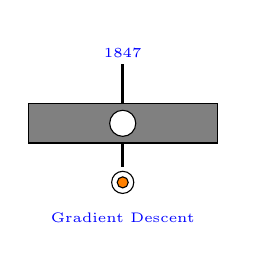
\begin{tikzpicture}[datemarker/.style={circle, draw=black,fill=white},textlabel/.style={anchor=center,text height=1.7ex,text depth=.25ex}]
					\tikzset{every node/.style={font=\tiny, color=blue}}\draw[fill=gray](-0.2,0) rectangle (2.2,0.5) node[white, below]{};
					\onslide<8->{\node at (1.0, 0.25) [datemarker] {};}
					\onslide<8->{\draw [line width=1pt] (1.0, 0.5) to (1.0, 1.0);}
					\onslide<8->{\draw (1.0, 1.2) node [textlabel] {1847 };}
					\onslide<8->{\draw [fill=orange](1.0, -0.5) circle (2pt){};}
					\onslide<8->{\draw (1.0, -0.5) circle (4pt){};}
					\onslide<8->{\draw [line width=1pt] (1.0, 0) to (1.0, -0.3);}
					\onslide<8->{\draw (1.0,-0.9) node [textlabel] {Gradient Descent};}
				\end{tikzpicture}
			\end{overlayarea}
			\column{0.9\textwidth}
			\begin{overlayarea}{\textwidth}{\textheight}
				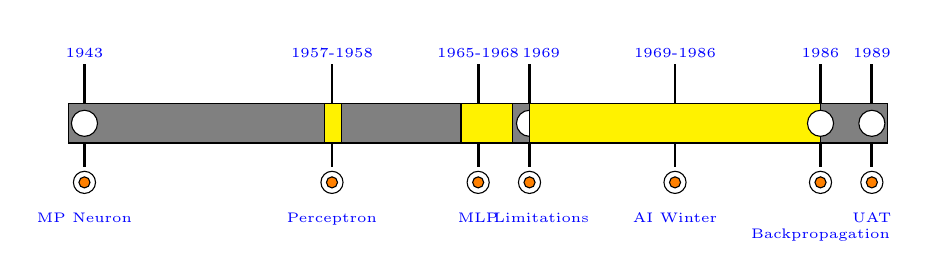
\begin{tikzpicture}[datemarker/.style={circle, draw=black,fill=white},textlabel/.style={anchor=center,text height=1.7ex,text depth=.25ex}]
					\tikzset{every node/.style={font=\tiny, color=blue}}\draw[fill=gray](-0.2,0) rectangle (10.2,0.5) node[white, below]{};
					\onslide<1->{\node at (0.0, 0.25) [datemarker] {};}
					\onslide<1->{\draw [line width=1pt] (0.0, 0.5) to (0.0, 1.0);}
					\onslide<1->{\draw (0.0, 1.2) node [textlabel] {1943 };}
					\onslide<1->{\draw [fill=orange](0.0, -0.5) circle (2pt){};}
					\onslide<1->{\draw (0.0, -0.5) circle (4pt){};}
					\onslide<1->{\draw [line width=1pt] (0.0, 0) to (0.0, -0.3);}
					\onslide<1->{\draw (0.0,-0.9) node [textlabel] {MP Neuron};}

					\onslide<2->{\draw[fill=yellow](3.04347826087, 0) rectangle (3.26086956522, 0.5){};}
					\onslide<2->{\draw [line width=1pt] (3.14347826087, 0.5) to (3.14347826087, 1.0);}
					\onslide<2->{\draw (3.14347826087, 1.2) node [textlabel] {1957-1958 };}
					\onslide<2->{\draw [fill=orange](3.14347826087, -0.5) circle (2pt){};}
					\onslide<2->{\draw (3.14347826087, -0.5) circle (4pt){};}
					\onslide<2->{\draw [line width=1pt] (3.14347826087, 0) to (3.14347826087, -0.3);}
					\onslide<2->{\draw (3.14347826087,-0.9) node [textlabel] {Perceptron};}


					\onslide<4->{\draw[fill=yellow](4.78260869565, 0) rectangle (5.4347826087, 0.5){};}
					\onslide<4->{\draw [line width=1pt] (5.0, 0.5) to (5.0, 1.0);}
					\onslide<4->{\draw (5.0, 1.2) node [textlabel] {1965-1968 };}
					\onslide<4->{\draw [fill=orange](5.0, -0.5) circle (2pt){};}
					\onslide<4->{\draw (5.0, -0.5) circle (4pt){};}
					\onslide<4->{\draw [line width=1pt] (5.0, 0) to (5.0, -0.3);}
					\onslide<4->{\draw (5.0,-0.9) node [textlabel] {MLP};}


					\onslide<5->{\node at (5.65217391304, 0.25) [datemarker] {};}
					\onslide<5->{\draw [line width=1pt] (5.65217391304, 0.5) to (5.65217391304, 1.0);}
					\onslide<5->{\draw (5.80217391304, 1.2) node [textlabel] {1969 };}
					\onslide<5->{\draw [fill=orange](5.65217391304, -0.5) circle (2pt){};}
					\onslide<5->{\draw (5.65217391304, -0.5) circle (4pt){};}
					\onslide<5->{\draw [line width=1pt] (5.65217391304, 0) to (5.65217391304, -0.3);}
					\onslide<5->{\draw (5.80217391304,-0.9) node [textlabel] {Limitations};}

					\onslide<6->{\draw[fill=yellow](5.65217391304, 0) rectangle (9.34782608696, 0.5){};}
					\onslide<6->{\draw [line width=1pt] (7.5, 0.5) to (7.5, 1.0);}
					\onslide<6->{\draw (7.5, 1.2) node [textlabel] {1969-1986};}
					\onslide<6->{\draw [fill=orange](7.5, -0.5) circle (2pt){};}
					\onslide<6->{\draw (7.5, -0.5) circle (4pt){};}
					\onslide<6->{\draw [line width=1pt] (7.5, 0) to (7.5, -0.3);}
					\onslide<6->{\draw (7.5,-0.9) node [textlabel] {AI Winter};}

					\onslide<7->{\node at (9.34782608696, 0.25) [datemarker] {};}
					\onslide<7->{\draw [line width=1pt] (9.34782608696, 0.5) to (9.34782608696, 1.0);}
					\onslide<7->{\draw (9.34782608696, 1.2) node [textlabel] {1986 };}
					\onslide<7->{\draw [fill=orange](9.34782608696, -0.5) circle (2pt){};}
					\onslide<7->{\draw (9.34782608696, -0.5) circle (4pt){};}
					\onslide<7->{\draw [line width=1pt] (9.34782608696, 0) to (9.34782608696, -0.3);}
					\onslide<7->{\draw (9.34782608696,-1.1) node [textlabel] {Backpropagation};}

					\onslide<9->{\node at (10.0, 0.25) [datemarker] {};}
					\onslide<9->{\draw [line width=1pt] (10.0, 0.5) to (10.0, 1.0);}
					\onslide<9->{\draw (10.0, 1.2) node [textlabel] {1989 };}
					\onslide<9->{\draw [fill=orange](10.0, -0.5) circle (2pt){};}
					\onslide<9->{\draw (10.0, -0.5) circle (4pt){};}
					\onslide<9->{\draw [line width=1pt] (10.0, 0) to (10.0, -0.3);}
					\onslide<9->{\draw (10.0,-0.9) node [textlabel] {UAT};}
				\end{tikzpicture}
			\end{overlayarea}
		\end{columns}
	\end{minipage}
\end{frame}
